%TODO: Less direct binding to previous section in introduction.
Now that a parallel k-d tree build algorithm has been build, lets start looking into a parallelization of the All-kNN operation. Some question immediately arise. What is the best way to parallelize such a problem? Will a GPU version give a beneficial speedup? This leads to a new research question that acts as an extension of RQ~\ref{rq:serial-kd-tree}.
%TSI requires high performance on repeated queries, how can we parallelize the All-kNN problem. something, something...

\begin{myrq}
\label{rq:parallel_query}
    It is possible to parallelize the All-kNN query algorithm, in such a way that it gives a significant speed improvement compared to the serial algorithm.
\end{myrq}

To investigate RQ~\ref{rq:parallel_query}, a real world test and implementation is always beneficial, but first some resource and discussion is needed. Especially in what kind of parallelization strategy and algorithm that should be used. Maybe the GPU is not the right way to parallelize this kind of operations.

\subsection{Parallelization strategy} % (fold)
\label{sub:parallelization_strategy}

Solving the All-kNN problem, can be done by repeated application of the kNN query algorithm. This is an algorithm that is easily parallelized, by distributing individual kNN queries across the available parallel units. However, there are still some possible pitfalls to address. Should a query be done in one block, maybe each query should be done single handedly by one thread, or maybe we should use one thread per $k$ in a query.

We have previously determined that a single query on a k-d tree size $m$, will in average visit $log(m)$ nodes. This indicates that not a lot of GPU resources is needed to perform a individual query. Assigning an entire CUDA block to one query therefore seems excessive. Combined with the communication heavy nature of the query algorithm, the best parallelization strategy is therefore to use one thread per query and equally distribute the queries amongst the GPU's SM\@.

Let us now consider if we can use Algorithm~\ref{alg:recursive_knn_kd_tree_search} directly with this parallelization strategy. As discussed in previous sections, GPUs and recursion don't get along well, the main drawback being the inherent need for communication between the recursive calls. Unfortunately, even with our current parallelization strategy, there are still reasons not to use a recursive algorithm. 

The GPU threads are lightweight, with restricted available memory and cache. This means that the call stack, where the all program instructions are managed, is relatively small. Given a non tail-recursive algorithm, the program context and instructions are appended to the call stack at each recursive call. This will eventually fill up the limited call stack available for an individual CUDA thread. It might be possible to still use a recursive algorithm, given that the call stack never gets to large.

% TODO: Fix verb tense
To determine if the recursive k-d tree query algorithm can fit within the CUDA thread call stack tests was performed. On a individual block, $64$ theoretical threads was spawned, querying a tree of increasing size. The results showed that when the tree size passed \numprint{1e5} points, unknown errors started to appear. This was probably caused by leak of call stack space.

Divergence also needs to be considered. In a recursive algorithm the decision of whether a recursive call should be made or not, is entirely up to a single thread. Once two threads have made different decisions, there is no guaranty that they will stay synchronized.

Both problems would be solved by rewriting Algorithm~\ref{alg:recursive_knn_kd_tree_search} into an iterative algorithm.
% end subsection parallelization_strategy (end)

\subsection{From recursive to iterative implementation} % (fold)
\label{sub:from_recursive_to_iterative_implementation}

% TODO: Explain combination of preoder and inorder dfs need.
To rewrite Algorithm~\ref{alg:recursive_knn_kd_tree_search} into a iterative algorithm by explicitly managing the recursion stack, some properties about how the search traverse the k-d tree is needed. From Algorithm~\ref{alg:recursive_knn_kd_tree_search} one can see that this is an inorder traversal, since the work of the current node is done between the recursive calls. This traversal in also the best strategy in a binary tree search, because the pruning of subtrees is maximized. How to make a standard binary search tree in an iterative fashion is described in Cormen\citep[Chapter 12]{Cormen:2001}, but since this is a k-d tree search the implementation is slightly different, as shown in Algorithm~\ref{alg:iterative_knn_kd_tree_search},

\begin{algorithm}
\caption{Iterative kNN k-d tree search}
\label{alg:iterative_knn_kd_tree_search}
\begin{algorithmic}
    \Procedure{Iterative-kNN-KD-Tree}{$K, r, q$}
        \State \text{Let $S$ be a stack for collecting tree nodes}

        \State $i \gets 2$

        \While{$!S.empty$ \textbf{or} $r$ != NIL}
            \If{$r$ = NIL}
                \State $r \gets \Call{Pop}{S}$
                \State $i \gets r.dimension$

                \If{$r.dx^2 < K.max$} \Comment{Can there be closer points in the other subtree?}
                    \State $r \gets r.other$
                \Else
                    \State $r \gets \text{NIL}$
                \EndIf
            \Else
                \State $d \gets \Call{Distance}{r, q}$

                \If{$d < K.max$} \Comment{Is $r$ closer to $q$ than the current k best points?}
                    \State $r.distance \gets d$
                    \State $\Call{Insert}{K, r}$
                \EndIf

                \State $i \gets (i + 1) \bmod k$ \Comment{k = 3 for a three dimensional k-d tree}

                \State $r.dimention \gets i$
                \State $r.dx \gets r.x(i) - q.x(i)$

                \If{$r.dx > 0$}  \Comment{Select $t$ and $o$ so we traverse towards closest point first}
                    \State $t \gets r.left$, $r.other \gets r.right$
                \Else
                    \State $t \gets r.right$, $r.other \gets r.left$
                \EndIf

                \State $\Call{Push}{S, r}$
                \State $r \gets t$
            \EndIf

        \EndWhile
    \EndProcedure
\end{algorithmic}
\end{algorithm}

The algorithm works in the same way as the recursive algorithm, but adds a stack, $S$, called the s-stack, and a while loop in order to handle the tree traversal iteratively. While there is a element assigned to the root variable, $r$, the algorithm will traverse down the target branch, updating the dimension, $i$, calculating the distance, $dx$, determining the target, $t$, and other, $o$, child node. Then it will collect $r$, $o$, $i$ and $dx$ into one element, and push it on the s-stack. Finally the root variable is assigned to the target child, or NIL if we have reached the end of a branch.

While there still is elements in the s-stack, but $r$ is assigned to NIL, we are traversing back up a branch. While this is happening, the algorithm pops elements from the s-stack, determines if they should be added to the k-heap, before it determines if it need to investigate the other branch of this node. If that is the case, the other node is assigned to $r$, and the algorithm will traverse down this subtree using the previously stated rules.
% subsection from_recursive_to_iterative_implementation (end)

\subsection{CUDA implementation} % (fold)
\label{sub:the_implementation}

Our simple parallelization strategy, combined with an iterative implementation of the k-d tree search algorithm, resulted in a trivial CUDA implementation, as we did not need to parallelize the iterative search algorithm itself. The implementation can be found in it's entirety in Appendix~\ref{sec:cuda_k_d_tree_search}. In addition, we will highlight some implementation details, and look at the results obtained from this code.

Algorithm~\ref{alg:iterative_knn_kd_tree_search} does not have a lot of divergence, and the remaining branching can be further reduced. If threads in a warp is traversing completely different parts of the tree, they will access different nodes. This is called data divergence. The solution is to let each warp search for points that are located closely in the k-d tree. This will cause all the threads to traverse down the tree in roughly along roughly the same branch, reducing the data divergence. Due to the nature of our k-d tree implementation, this can be achieved by feeding the points to the search algorithm as they are placed in the k-d tree.

%TODO: Possible citation 400-600$ clock cycles.
The explicit stack also makes an interesting question about where to store the new stack. This is data that are modifiable and thread independent, which means that the possible options memory options are shared memory, local memory and global memory. Local memory is the memory each thread can allocate dynamically from the heap. Global memory is a possible candidate. It has enough space, it is modifiable and accessible to all threads. The drawback is the access time, it takes around $400-600$ clock cycles, and it would therefore be beneficial to use some other kind of memory. Shared memory would be a perfect candidate, because the memory is fast and the need to communicate between blocks is nonexistent. The only drawback is the amount of data available in shared memory, which is around $49 kb$ on current NVIDIA GPU's. 

The iterative search algorithm uses one stack and one heap, both stored as arrays in memory. Th number of arrays are dependent on the number of threads used in each block. The s-stack array size is dependent on how many elements the inorder tree traversal needs to store. If one looks on how the algorithm handles the stack, one can see that elements are pushed on the way down, and poped on the way up. This means that the stack never will be longer then the tree hight. One stack element uses $16$ bytes of space, which means that the stack memory is s subset of $\Theta(16\log_2(n)T)$. Here $T$ represent the number of threads and $n$ is the k-d tree size. The k-heap array size, depends on the number of closest neighbors, $k$, and one element uses $8$ bytes. This implies that it's memory usage will be, $\Theta(8kT)$.

\begin{figure}[ht!]
\centering
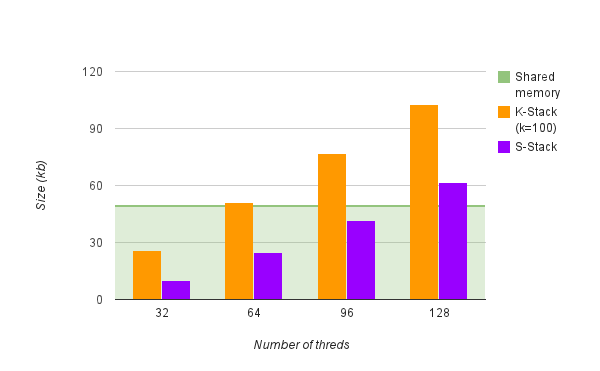
\includegraphics[width=100mm]{../gfx/shared_memory_and_stack.png}

\caption{The stacks memory usage, compared to the amount of shared memory. Here $k$ was sat to $100$.}
\label{fig:stacks_and_shared_memory}
\end{figure}

In Figure~\ref{fig:stacks_and_shared_memory} the memory usage of each stack is compared to the available shared memory. Some basic assumptions and approximations have been done in regard to the data. Treads are only compared in multiples of $32$, since this is the warp size and is therefore the most optimal thread numbers. The value of $k$ is dependent on the problem in hand, and as our application only needs a value of $100$, so that value is used. 

%TODO: k-stack -> k-heap in figure
Figure~\ref{fig:stacks_and_shared_memory} shows that the k-heap will not fit in shared memory. Already at a thread count of $64$ the memory is filled up. The size of the k-heap is also highly dependent on the size of $k$ which is hard to predict. However, locating the s-stack on shared memory looks promising. The memory size has also a relatively low asymptotic growth, \BigO{log(n)}, in regard to the tree size.

\begin{figure}[ht!]
    \centering
    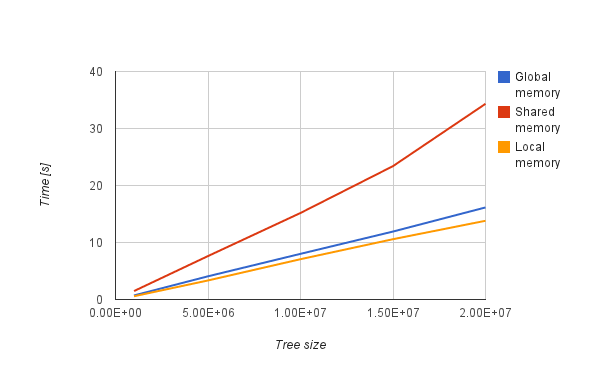
\includegraphics[width=100mm]{../gfx/stack_speed.png}

    \caption{Search time comparison between different stack memory types. The test are done with $k$ equals 10 and \numprint{1e6} queries per tree size. }
    \label{tbl:stack_speed}
\end{figure}

To decide what kind of memory is optimal location for the s-stack, Figure~\ref{tbl:stack_speed} has been created. Surprisingly shared memory looks like the slowest alternative. One likely reason is that elements in shared memory is synced between all threads in a block. This property is not needed in the s-stack, since the s-stack is only used by one thread.

Although global and local memory presumably is stored at the same place, the are some noticeable differences that can explain the time gap between them. The cache may be a factor. The cache is placed on the same on-chip memory as the shared memory, and should therefore be equally fast. The difference is that cashing is not programmable and therefor not controlled be the programmer. However some properties in the local memory may suggest that it is a more likely candidate to be cached. The local memory is thread dependent and is not accessible to other threads or blocks as the global memory are. The compiler can therefor logically imply that the data is not going to be modified by other threads and caching becomes much more likely. Figure~\ref{fig:stacks_and_shared_memory}, also shows us that the cache can fit the hole s-stack in a block, which correlates with the timing results. To enforce cache use even further, CUDA gives a runtime option to enforce more of the on-chip memory to caching.

\begin{figure}[ht!]
    \centering
    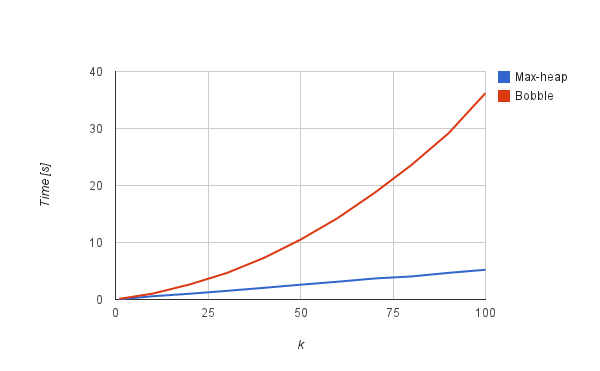
\includegraphics[width=100mm]{../gfx/k_stack.png}

    \caption{Timing results from two different k-heap implementations, with varying $k$ and \numprint{1e6} referance points. }
    \label{tbl:k_stack}
\end{figure}

Testing different memory locations for the s-stack, showed that the memory location is important for performance. Even small improvements in the performance of the s-stack, gives a significant improvement in overall runtime. This implies that the k-heap should be highly optimized.

Figure~\ref{tbl:k_stack} shows the runtime difference between two k-heap variants. One uses a bobble sort\cite{Cormen:2001} like implementation. It works by always keeping a sorted list. Elements are inserted by placing it at the end if the list, and swapping it to the adjustment element, until it is in the right place. The other method is based on a heap sort implementation, that is explained in Section~\ref{sub:querying_the_k_d_tree}. The performance difference is the insertion time, where the bobble variant is a \BigO{n} time complexity, while heap sort variant has a \BigO{log_2(n)}. Resulting in a almost $7$ times faster k-heap, with only a $k$ value of $100$.
% subsection the_implementation (end)

\subsubsection{Open-MP} % (fold)
\label{ssub:open_mp_version}

The high impact the stack had on performance make an interesting question in regard to RQ~\ref{rq:parallel_query}. Could a parallel implementation on the CPU outperform the CPU version? When the latency effect, as the stacks showed, had such a huge impact on the performance. The CPU has a lot more cache then the GPU and would therefor not be affected that much by memory overhead. The question if this is enough to offset the lower number of parallel threads on the CPU.

For this to be investigated properly, an OpenMP version of the k-d tree search has to be created. The parallelization strategy is the same as for the CUDA implementation, only differing in implementation details. Since the CPU has vastly more cache and the system memory latency is not very high, we do not need to consider memory usage in the same manner as with the CUDA implementation. The implementation can be found in Appendix~\ref{sec:open_mp_k_d_tree_search}.
% subsubsection open_mp_version (end)
% subsection our_implementation (end)
